Код, используемый для построения графов:

\begin{verbatim}
1. ingridients := strings.Split(str, ";")
2. for _, ing := range ingridients {
3. 	start := -1
4. 	end := -1
5. 	for i, r := range ing {
6. 		if (r >= '0' && r <= '9') || r == '-' || r == '.' {
7. 			if start == -1 {
8. 				start = i}
9. 		} else if start != -1 {
10. 			end = i
11. 			break}}
12. 	if start != -1 && end == -1 {
13. 		end = len(ing)}
14. 	if start == -1 {
15. 		name, unit, qty = ing, "", ""
16. 	} else {name = ing[:start], unit = ing[start:end],
qty = ing[end:]}
17. 	task.Data.Ingredients = append(task.Data.Ingredients,
tasks.Ingredient{Name: name, Unit: unit, Quantity: qty})}
\end{verbatim}

Входные данные для ОИ и ИИ:

\begin{verbatim}
str = "У;Л 2 ш;И 3;Ж п 0.5 кг;"
\end{verbatim}

\begin{figure}[H]
    \centering
    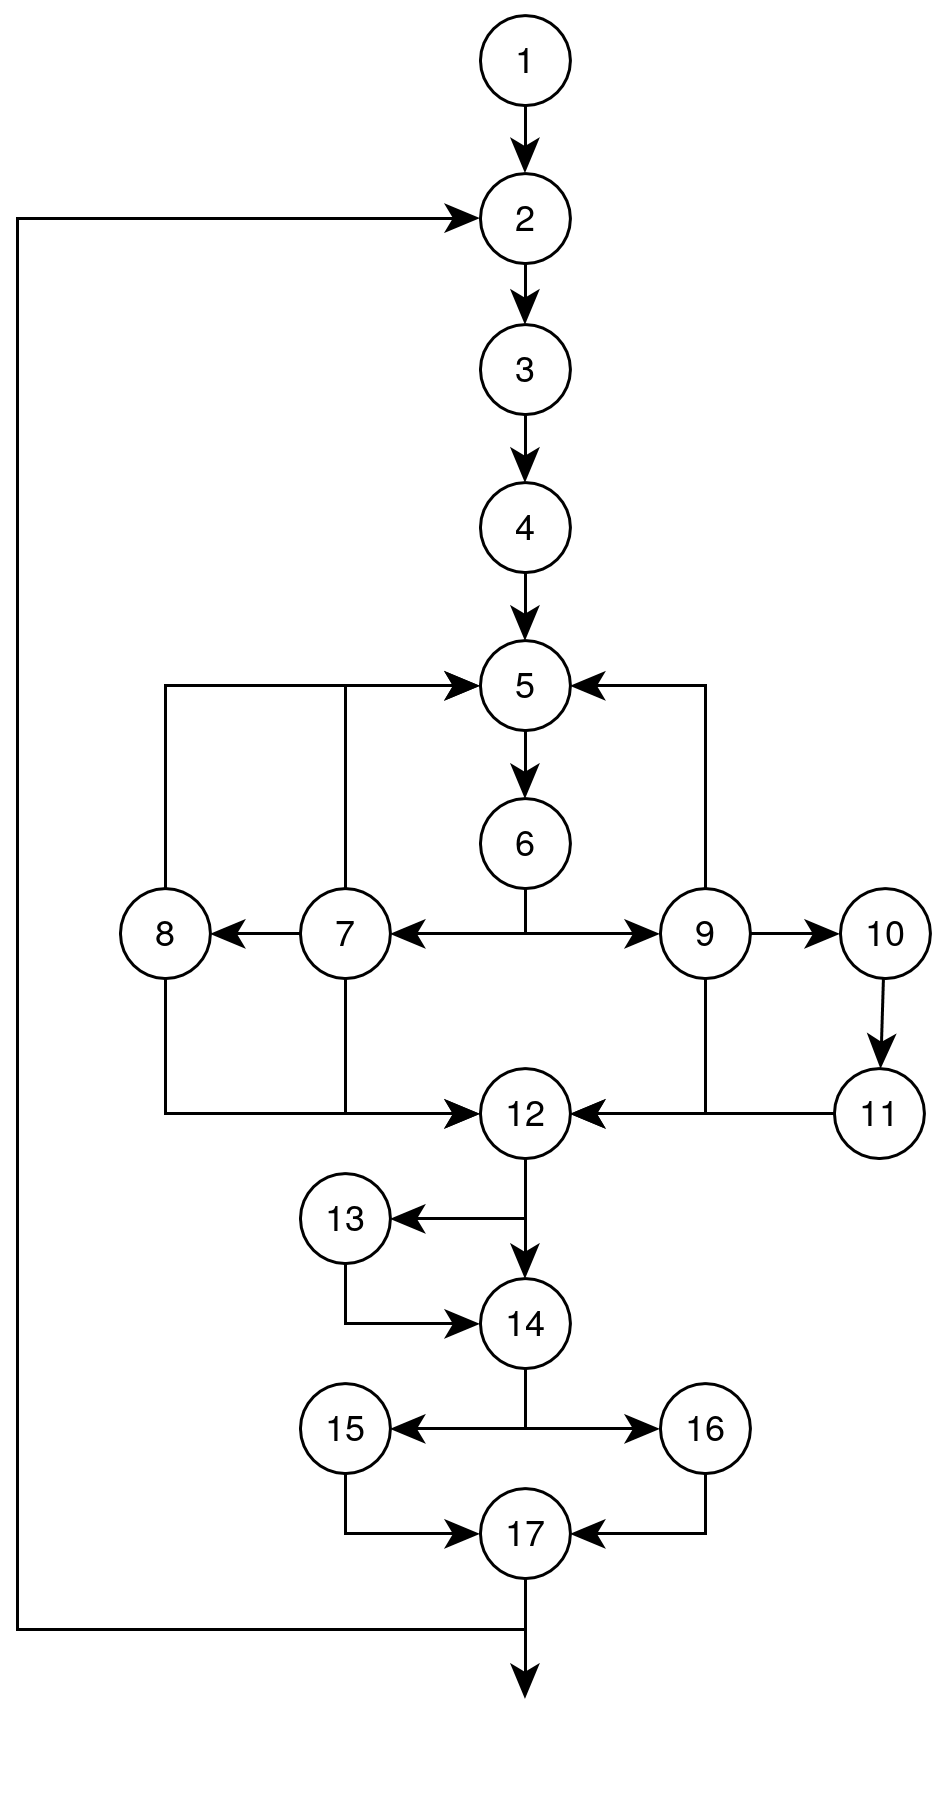
\includegraphics[scale=0.3]{img/GU.png}
    \caption{Граф управления}
\end{figure}

\begin{figure}[H]
    \centering
    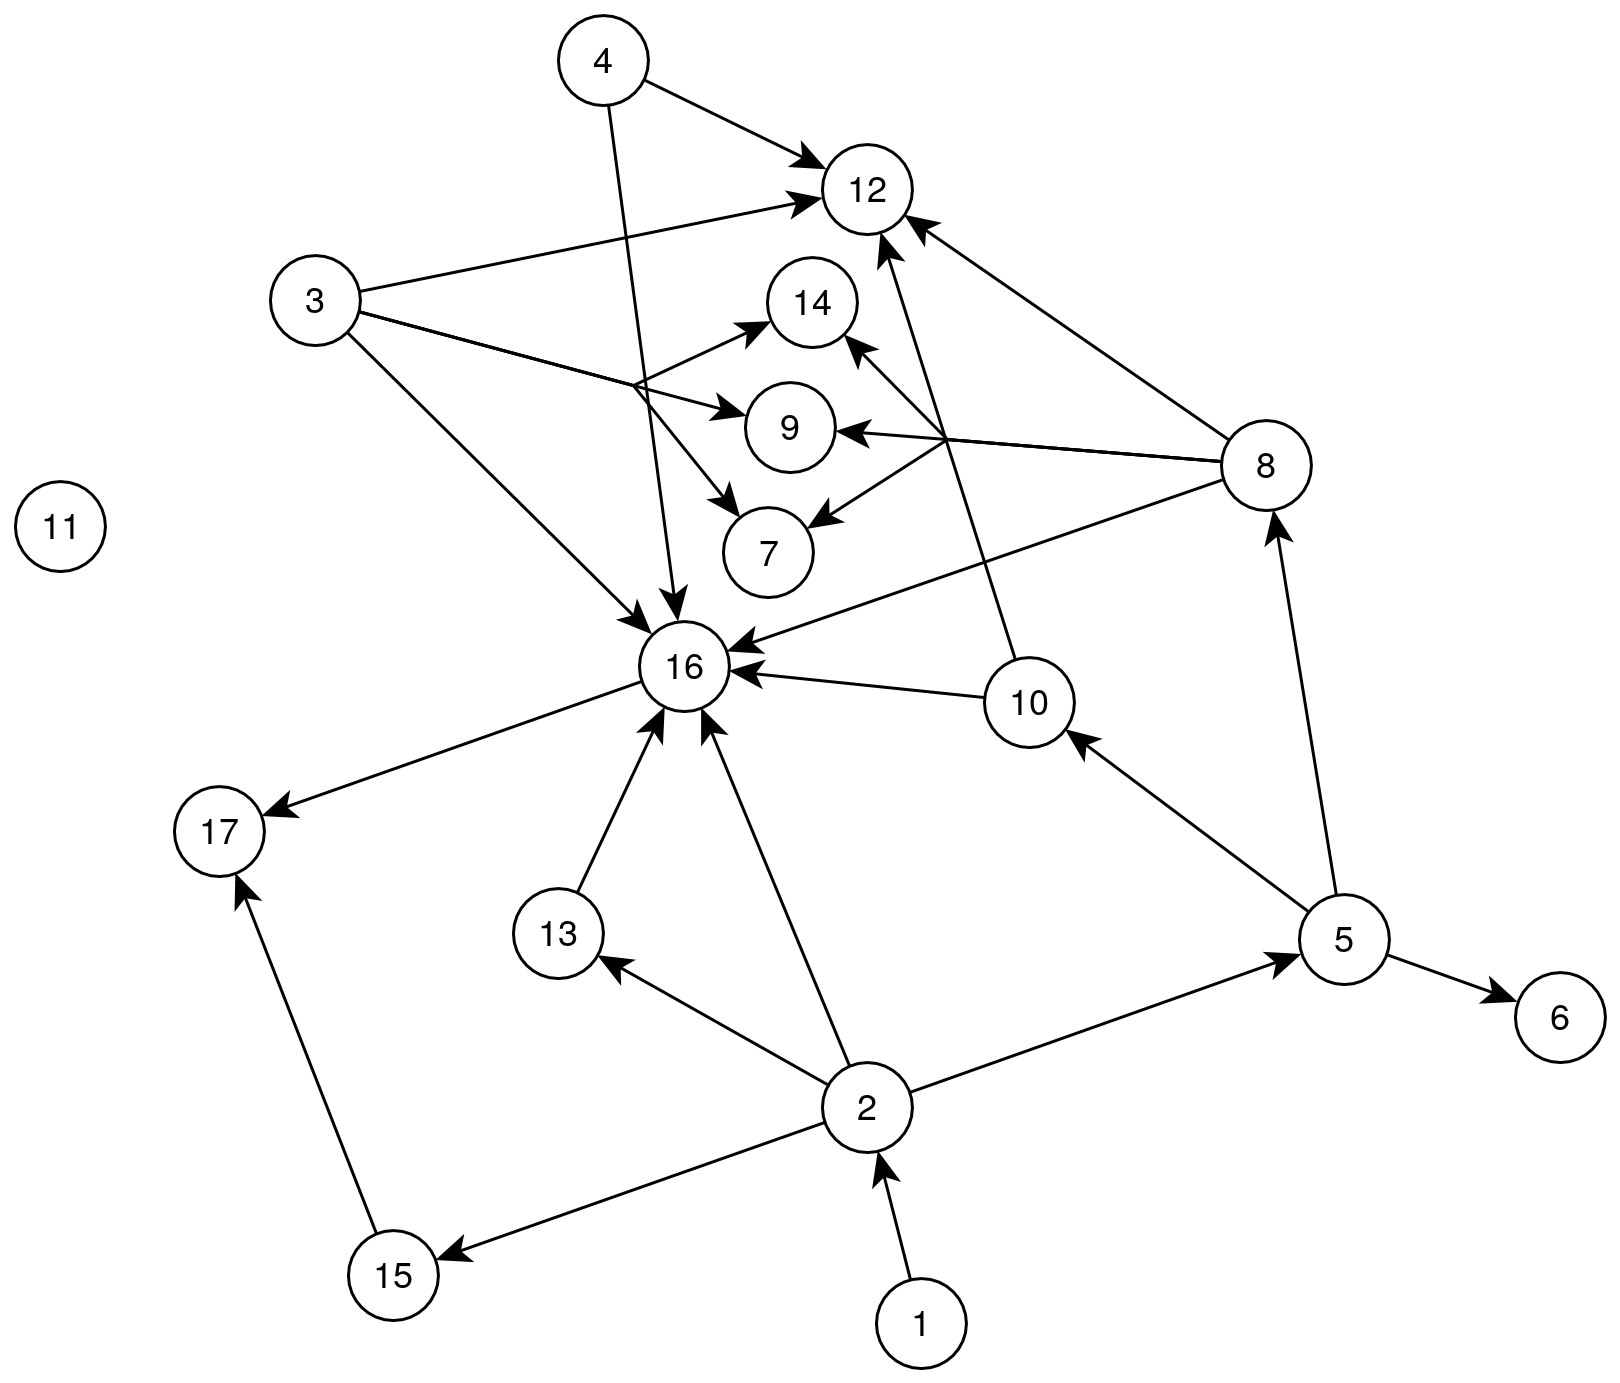
\includegraphics[scale=0.27]{img/IG.png}
    \caption{Информационный граф}
\end{figure}

\begin{figure}[H]
    \centering
    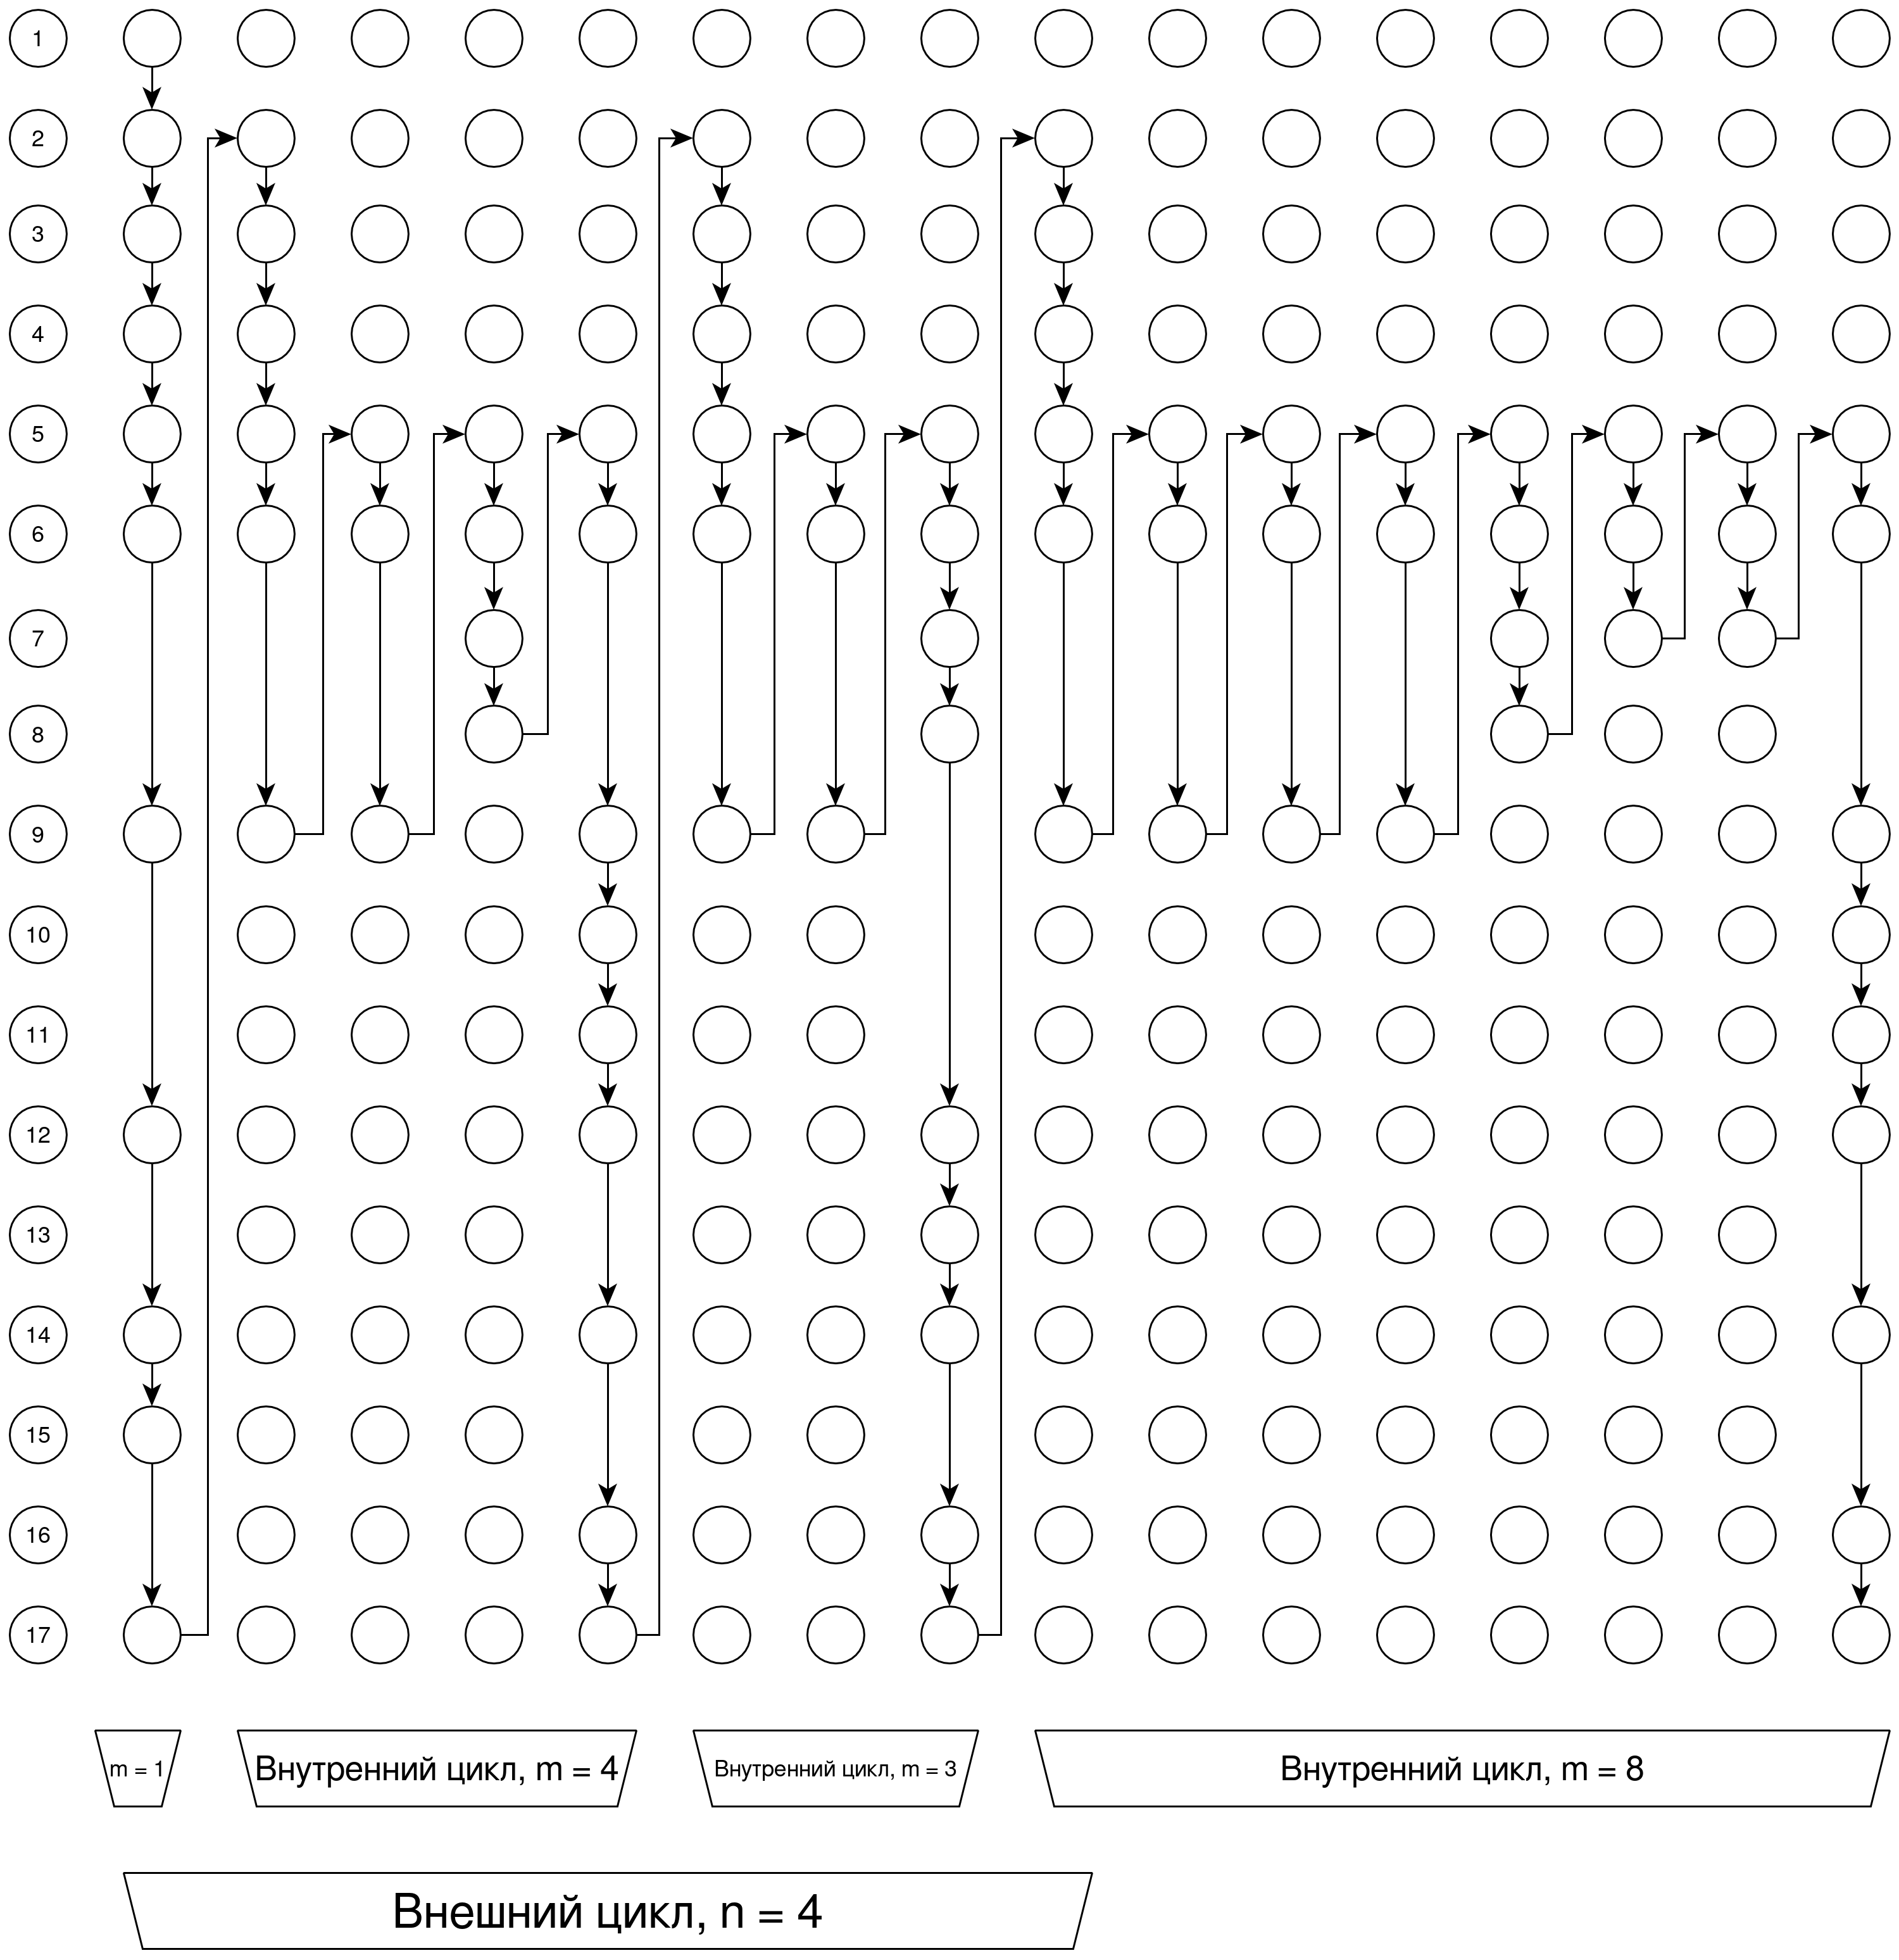
\includegraphics[scale=0.15, angle=90]{img/OI.png}
    \caption{Операционная история}
\end{figure}

\begin{figure}[H]
    \centering
    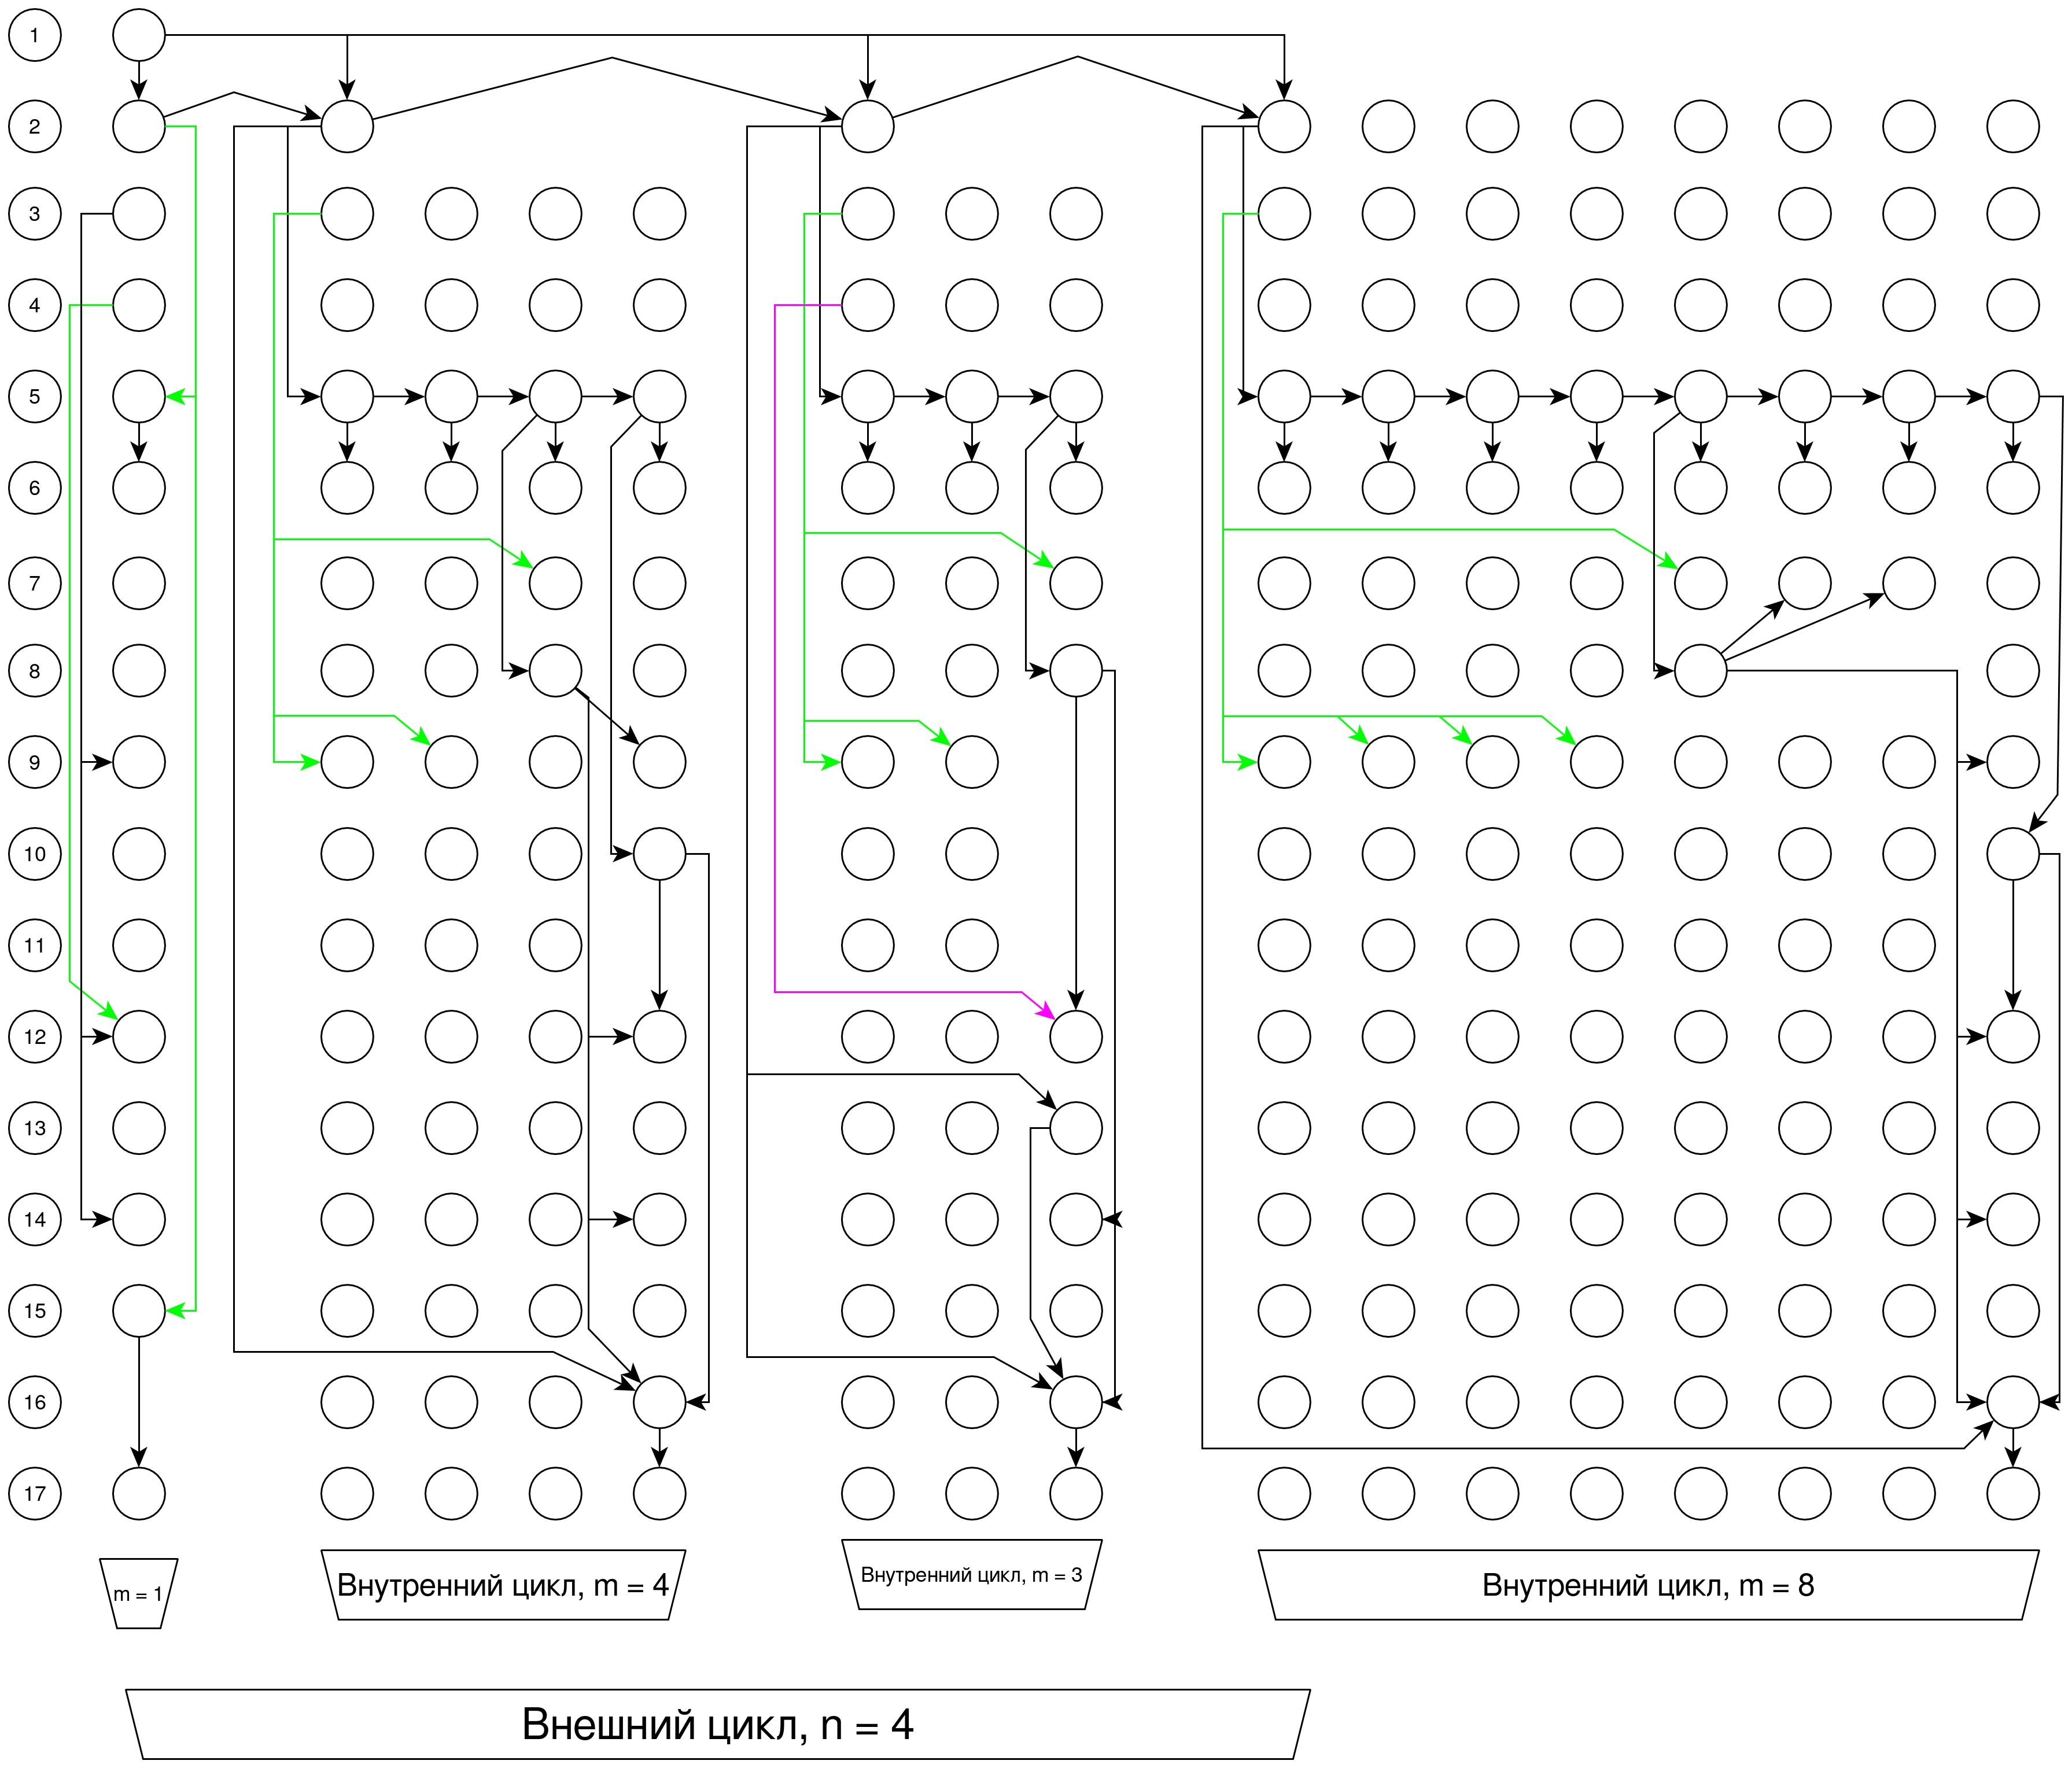
\includegraphics[scale=0.15, angle=90]{img/II.png}
    \caption{Информационная история}
\end{figure}

